% !TeX TXS-program:compile = txs:///pdflatex/[--shell-escape]

\documentclass[11pt, letterpaper]{article}

\usepackage{minted}
\usepackage[utf8]{inputenc}
\usepackage[T1]{fontenc}
\usepackage{lmodern}
\usepackage{graphicx}
\usepackage{longtable}
\usepackage{wrapfig}
\usepackage{rotating}
\usepackage{amsmath}
\usepackage{textcomp}
\usepackage{amssymb}
\usepackage{hyperref}
\usepackage[round]{natbib}
\usepackage{subcaption}


\title{\bfseries Tarea}
\author{Ángel García Báez}
\date{\today}
\setcounter{tocdepth}{3} 

\begin{document}
	
	% Página de presentación
	\begin{titlepage}
		\centering
		
\includegraphics[width=0.2\textwidth]{logo.png}\par
		\vspace{1cm}
		{\LARGE \bfseries Universidad Veracruzana \par}
		\vspace{1cm}
		{\Large Maestría en Inteligencia Artificial\par}
		\vspace{3cm}
		{\LARGE \bfseries Visión por Computadora \par}
		\vspace{1cm}
		{\Large \bfseries Tarea 9. Segmentación de colores con espacios HSV y LAB MATLAB. \par}
		\vfill
		{\Large \textit{Ángel García Báez}\par}
		\vspace{1cm}
		{\Large Profesor: Dr. Héctor Acosta Mesa \par}
		\vfill
		{\Large \today \par}
	\end{titlepage}
	
	% Página exclusiva para la tabla de contenidos
	\newpage
	\tableofcontents
	\newpage
	
% Sección para el problema 1
\section{Objetivo de la práctica}

Para la presente practica, se desea poder implementar una función propia que tome una imagen y permita realizar la segmentación de los pixeles de la misma mediante una transformación del espacio de colores tradicional RGB a otros espacios como HSV y LAB para realizar dicha segmentación basandose unicamente en los canales de colores.

Para ello, la función debe permitir seleccionar cualquier pixel de la imagen para tomarlo como referencia para realizar la segmentación en busca de similaridades mediante un umbral fijado de la distancia de los pixeles de la imagen al pixel de referencia seleccionado.

Para llevar a cabo la practica se aplicara el proceso de segmentación sobre la siguiente imagen de la cantante Denisse Guerrero de Belanova, extraída de su cuenta de instagram oficial:


\begin{figure}[h!]
	\centering
	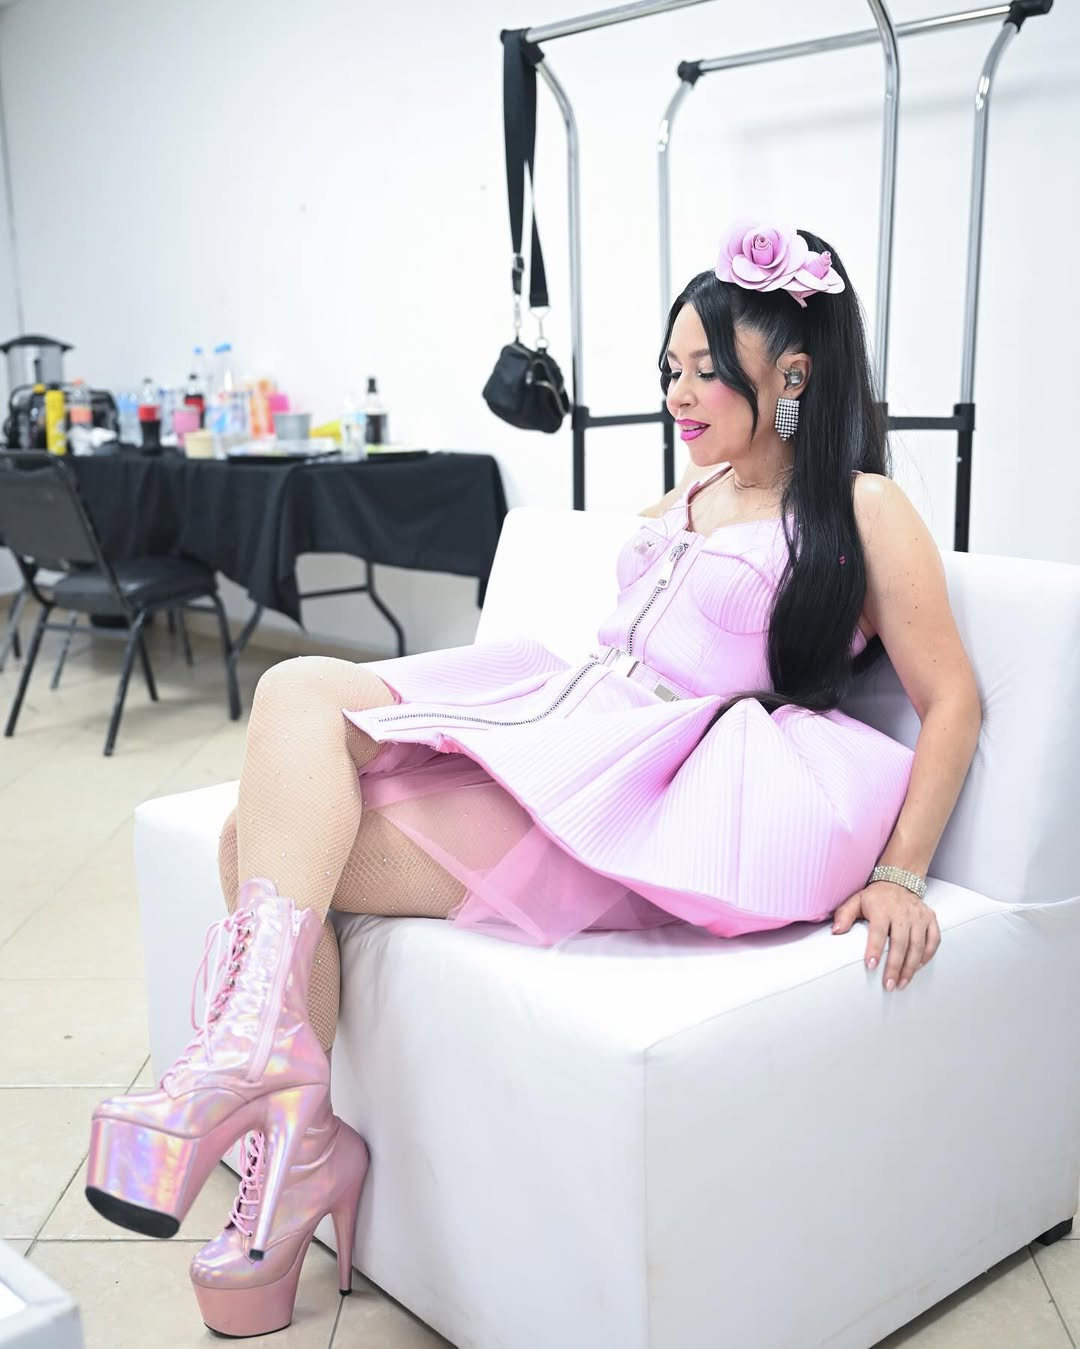
\includegraphics[width=0.5\textwidth]{IMG/IM4.jpeg}
	\caption{Foto de Denisse Guerrero.}
	\label{fig:r0_r1}
\end{figure}

	
\newpage
	
\section{Metodología}

De acuerdo con \cite{gonzalez2018digital}, un espacio de color es un modelo matemático que describe la representación de los colores en un formato que puede ser interpretado y procesado por sistemas computacionales o visualizado por humanos. Cada color dentro de un espacio está definido por un conjunto de coordenadas, normalmente en tres dimensiones, como en los espacios RGB, HSV o CIE L*a*b*. La elección del espacio de color afecta directamente la facilidad con que ciertas tareas de procesamiento de imagen, como la segmentación o el reconocimiento de objetos, pueden realizarse. \\

El espacio HSV (Hue, Saturation, Value) es un espacio de color perceptual diseñado para ser más intuitivo para los humanos que el modelo RGB. Está compuesto por tres componentes:


\begin{itemize}
	
	\item Hue (H): tonalidad del color, representada como un ángulo en el círculo cromático, en grados (0°–360°).
	
	\item Saturation (S): pureza del color, que varía de 0 (gris) a 1 (color completamente puro).
	
	\item Value (V): brillo del color, que varía de 0 (negro) a 1 (máxima luminosidad).
	
	
\end{itemize}



Este modelo es útil en aplicaciones como la segmentación por color, ya que permite separar el matiz de la intensidad de luz, facilitando tareas de procesamiento basadas en la percepción humana.

El espacio de color HSV (Hue, Saturation, Value) permite representar colores de forma más intuitiva que el espacio RGB, ya que separa las propiedades cromáticas del color (tono y saturación) de su brillo. Para convertir un color del espacio RGB al HSV, primero se normalizan los valores \( R, G, B \in [0,1] \), y luego se calculan:

\[
C_{\text{max}} = \max(R, G, B), \quad 
C_{\text{min}} = \min(R, G, B), \quad 
\Delta = C_{\text{max}} - C_{\text{min}}
\]

El matiz \( H \), medido en grados sobre el círculo cromático, se define como:

\[
H =
\begin{cases}
	0^\circ, & \text{si } \Delta = 0 \\
	60^\circ \cdot \left( \frac{G - B}{\Delta} \mod 6 \right), & \text{si } C_{\text{max}} = R \\
	60^\circ \cdot \left( \frac{B - R}{\Delta} + 2 \right), & \text{si } C_{\text{max}} = G \\
	60^\circ \cdot \left( \frac{R - G}{\Delta} + 4 \right), & \text{si } C_{\text{max}} = B
\end{cases}
\]

La saturación \( S \), que representa la intensidad o pureza del color, se calcula como:

\[
S =
\begin{cases}
	0, & \text{si } C_{\text{max}} = 0 \\
	\frac{\Delta}{C_{\text{max}}}, & \text{en otro caso}
\end{cases}
\]

El valor \( V \), que representa el brillo del color, es simplemente:

\[
V = C_{\text{max}}
\]

Este modelo resulta particularmente útil en procesamiento de imágenes y visión por computadora, especialmente en tareas como segmentación basada en color.



\begin{itemize}
	\item Primero se obtuvo el gráfico de los 1520 conjuntos de puntos correspondientes a sus imágenes y se graficaron.
	
	\item Segundo, se hizo el registro de cada uno de los 1520 conjuntos de puntos respecto a la imagen 1 y se graficaron. 
	
	\item Tercero, se obtuvo el ERM de cada conjunto de puntos transformado respecto al conjunto de la imagen 1 para evaluar que tan bueno fue el ajuste. Se hizo el histograma de la distribución de los errores cuadráticos medios y se ordenaron de menor a mayor.
	
	\item Finalmente, se obtuvieron unicamente los 100 conjuntos de puntos transformados que presentaron el error cuadrático más pequeño y se graficaron.
	
\end{itemize}

\begin{figure}[h!]
	\centering
	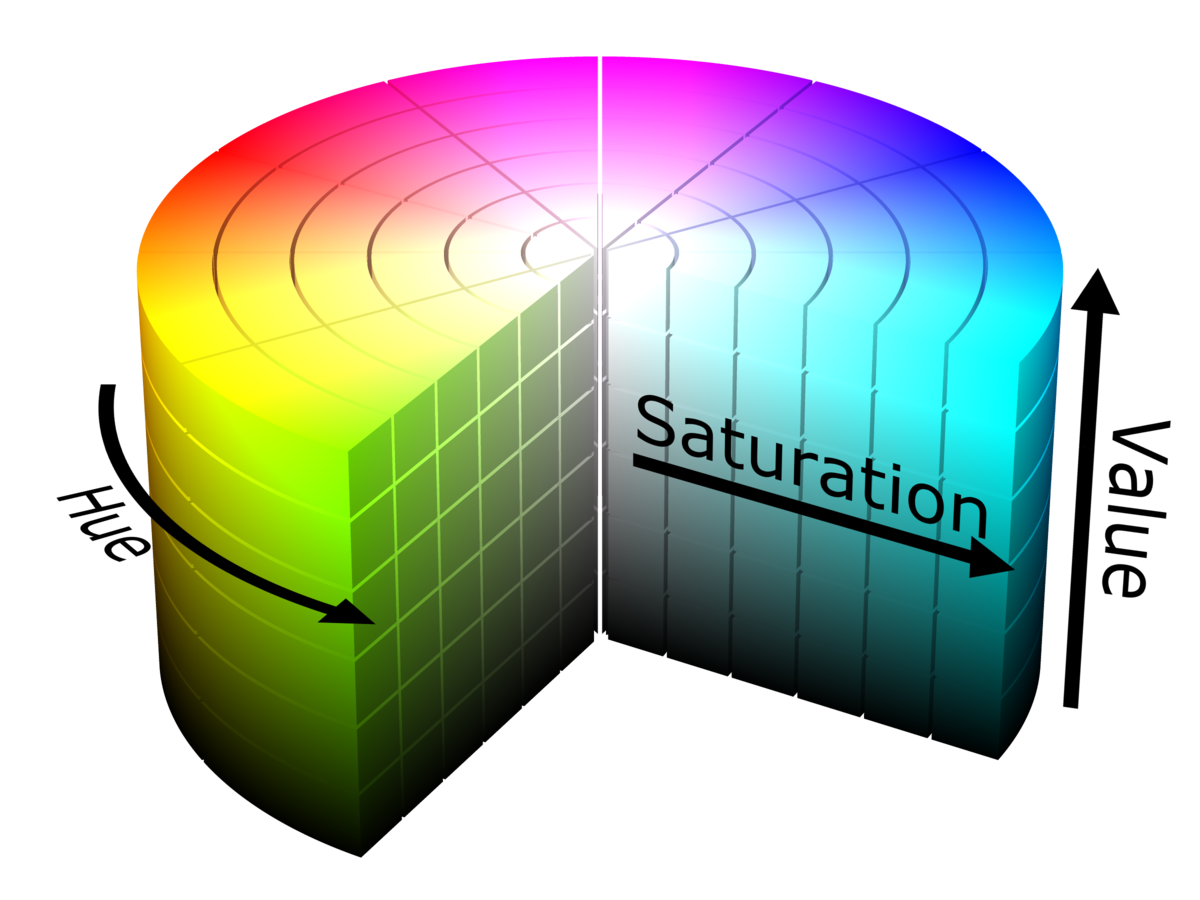
\includegraphics[width=0.5\textwidth]{IMG/REF1.png}
	\caption{Representación del espacio HSV.}
	\label{fig:r1}
\end{figure}

\newpage

Por otro lado, el espacio de color CIE L\*a\*b\* es un modelo perceptualmente uniforme propuesto por la Comisión Internacional de Iluminación (CIE) en 1976. Está diseñado para representar los colores de forma que la distancia euclideana entre dos colores se aproxime a la percepción humana de la diferencia entre ellos. El modelo se basa en un espacio tridimensional donde:

\begin{itemize}
	\item \( L^* \) representa la luminosidad (de 0 a 100).
	\item \( a^* \) representa la posición entre verde (valores negativos) y rojo (valores positivos).
	\item \( b^* \) representa la posición entre azul (valores negativos) y amarillo (valores positivos).
\end{itemize}

La representación de dicho espacio se puede observar como una esfera en 3 dimensiones:

\begin{figure}[h!]
	\centering
	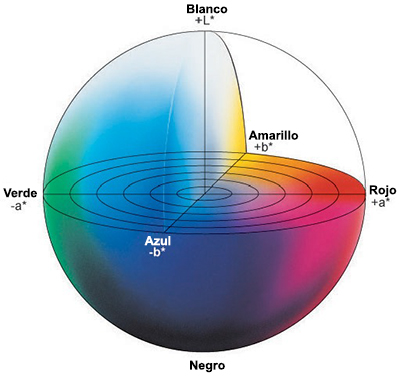
\includegraphics[width=0.5\textwidth]{IMG/REF2.jpg}
	\caption{Representación del espacio LAB.}
	\label{fig:r2}
\end{figure}


Para convertir de RGB a CIE L\*a\*b\*, primero se convierte RGB a XYZ (espacio de referencia absoluto), y luego XYZ a L\*a\*b\*. Los pasos son:

1. De RGB a XYZ: 
Primero se normaliza \( R, G, B \in [0,1] \) (si estaban en el rango \([0,255]\)), y se linealizan con:

\[
C_{\text{lin}} =
\begin{cases}
	\frac{C}{12.92}, & \text{si } C \leq 0.04045 \\
	\left( \frac{C + 0.055}{1.055} \right)^{2.4}, & \text{si } C > 0.04045
\end{cases}
\]

Luego, se calculan los valores XYZ usando la matriz de transformación para el espacio sRGB con iluminante D65:

\[
\begin{bmatrix}
	X \\
	Y \\
	Z
\end{bmatrix}
=
\begin{bmatrix}
	0.4124564 & 0.3575761 & 0.1804375 \\
	0.2126729 & 0.7151522 & 0.0721750 \\
	0.0193339 & 0.1191920 & 0.9503041
\end{bmatrix}
\cdot
\begin{bmatrix}
	R_{\text{lin}} \\
	G_{\text{lin}} \\
	B_{\text{lin}}
\end{bmatrix}
\]

2. De XYZ a CIE L\*a\*b\: 
Se normaliza respecto al blanco de referencia \( (X_n, Y_n, Z_n) \), y se define la función intermedia:

\[
f(t) =
\begin{cases}
	t^{1/3}, & \text{si } t > \delta \\
	\frac{t}{3\delta^2} + \frac{4}{29}, & \text{si } t \leq \delta
\end{cases}, \quad \text{donde } \delta = \left(\frac{6}{29}\right)^3
\]

Luego, los valores L\*a\*b\* se calculan como:

\[
L^* = 116 \cdot f\left(\frac{Y}{Y_n}\right) - 16
\]
\[
a^* = 500 \cdot \left[ f\left(\frac{X}{X_n}\right) - f\left(\frac{Y}{Y_n}\right) \right]
\]
\[
b^* = 200 \cdot \left[ f\left(\frac{Y}{Y_n}\right) - f\left(\frac{Z}{Z_n}\right) \right]
\]

Este espacio de color es muy usado en visión computacional y procesamiento de imágenes debido a su uniformidad perceptual.


Una vez definidos los conceptos necesarios, la metodología aplicada para la practica en lenguaje MATLAB consiste en lo siguiente:

\begin{itemize}
	\item Cargar la imagen en RGB.
	\item Seleccionar el espacio de color a donde va a ser mapeada la imagen original (HSV).
	\item Seleccionar un pixel de referencia de la imagen.
	\item Definir un umbral que permita marcar cuando un pixel de la imagen transformada se "parezca" o este cerca al pixel de referencia con respecto a la distancia euclidiana.
	\item Repetir el proceso de revisar con cada uno de los pixeles de la matriz hasta obtener la mascara de la imagen completa de los pixeles que se parecen al pixel de referencia
	\item Repetir en el espacio LAB
	
\end{itemize}

Nota: Se uso el mismo pixel de referencia para todas las segmentaciones.

\newpage
	
\section{Resultados}

\subsection{Segmentación en HSV con un umbral de 0.15}

\begin{figure}[h!]
	\centering
	\begin{minipage}{0.35\textwidth}
		\centering
		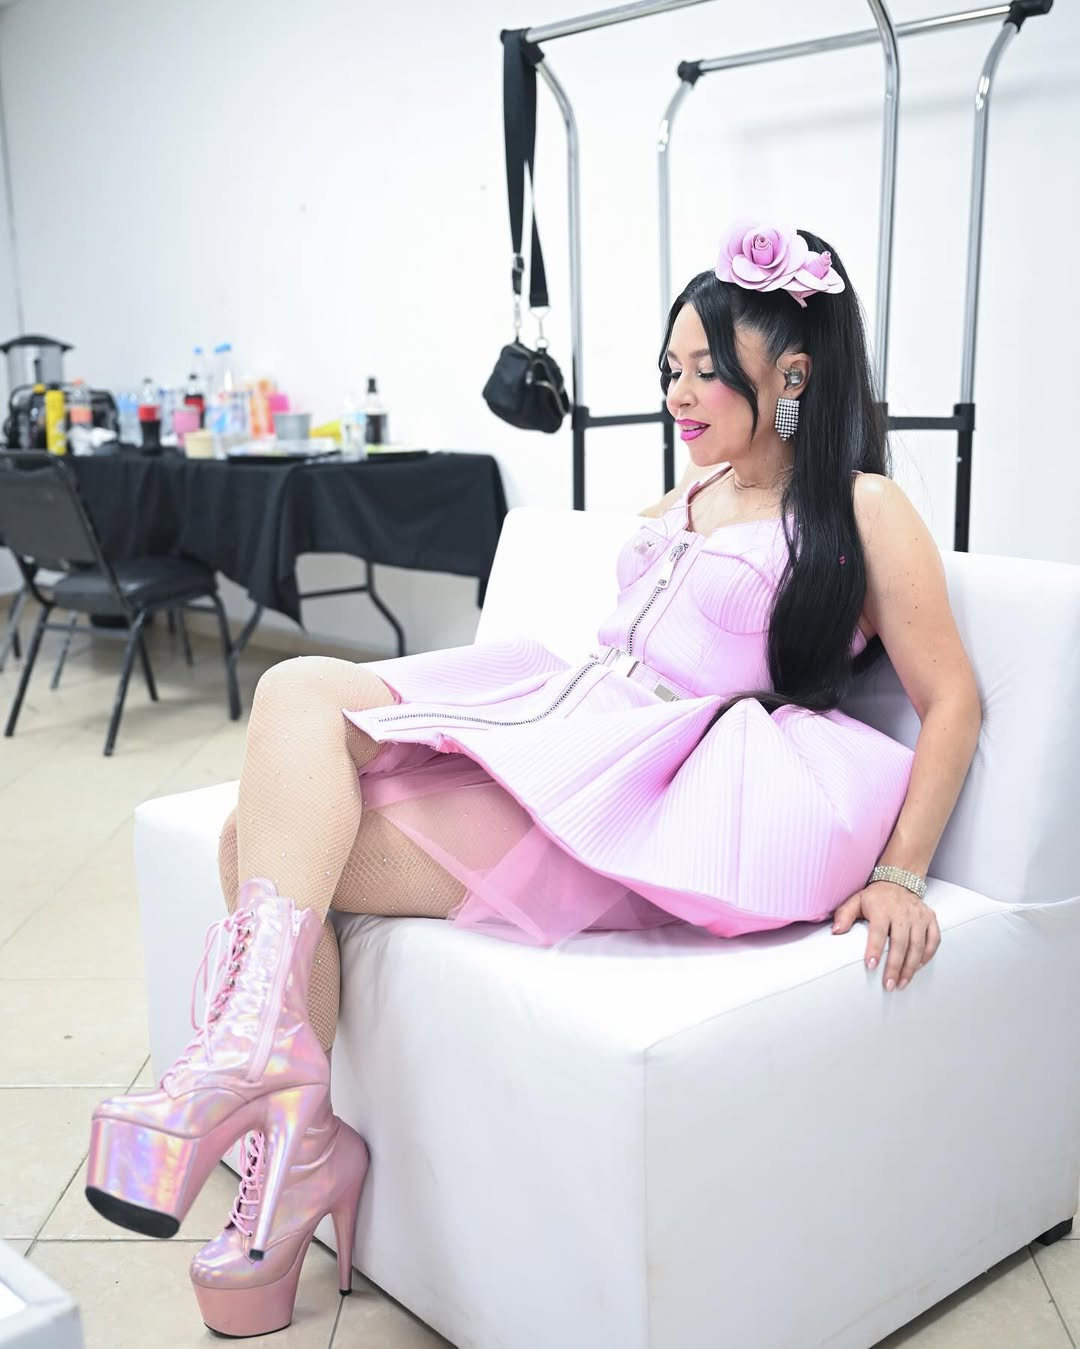
\includegraphics[width=\textwidth]{IMG/IM4.jpeg}
		\caption*{Imagen original.}
	\end{minipage}\hfill
	\begin{minipage}{0.35\textwidth}
		\centering
		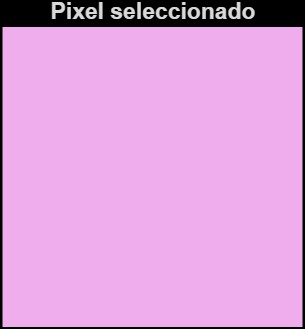
\includegraphics[width=\textwidth]{IMG/PIXEL.jpg}
		\caption*{Pixel seleccionado para la segmentación.}
	\end{minipage}
	
	\vspace{1em} % Espacio vertical entre las filas
	
	\begin{minipage}{0.35\textwidth}
		\centering
		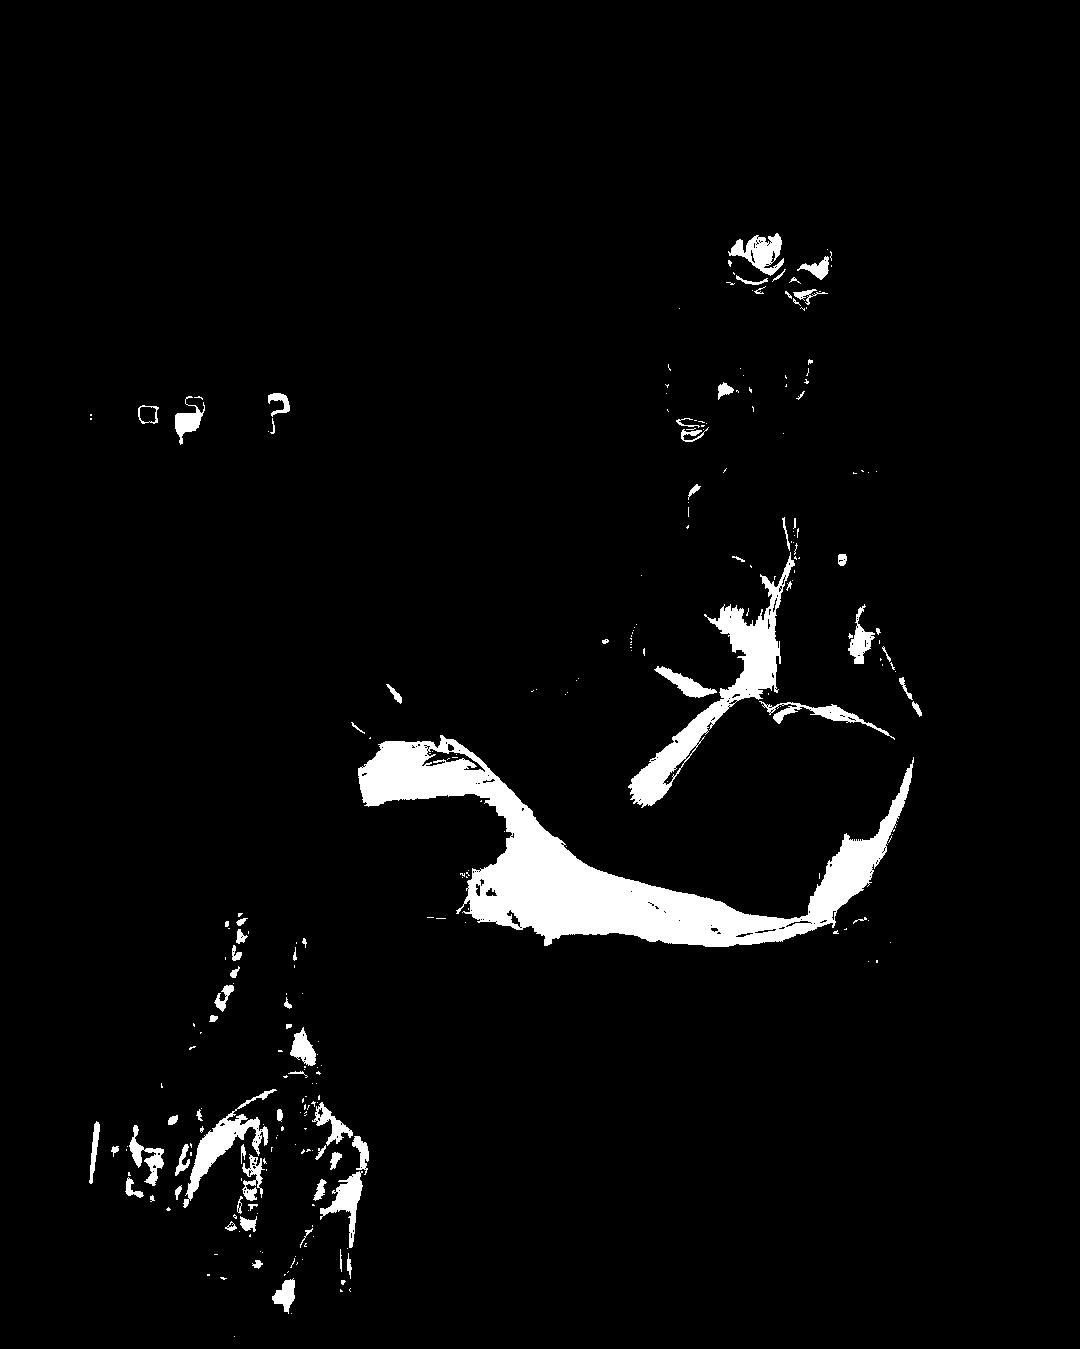
\includegraphics[width=\textwidth]{IMG/R12.jpg}
		\caption*{Mascara seleccionada.}
	\end{minipage}\hfill
	\begin{minipage}{0.35\textwidth}
		\centering
		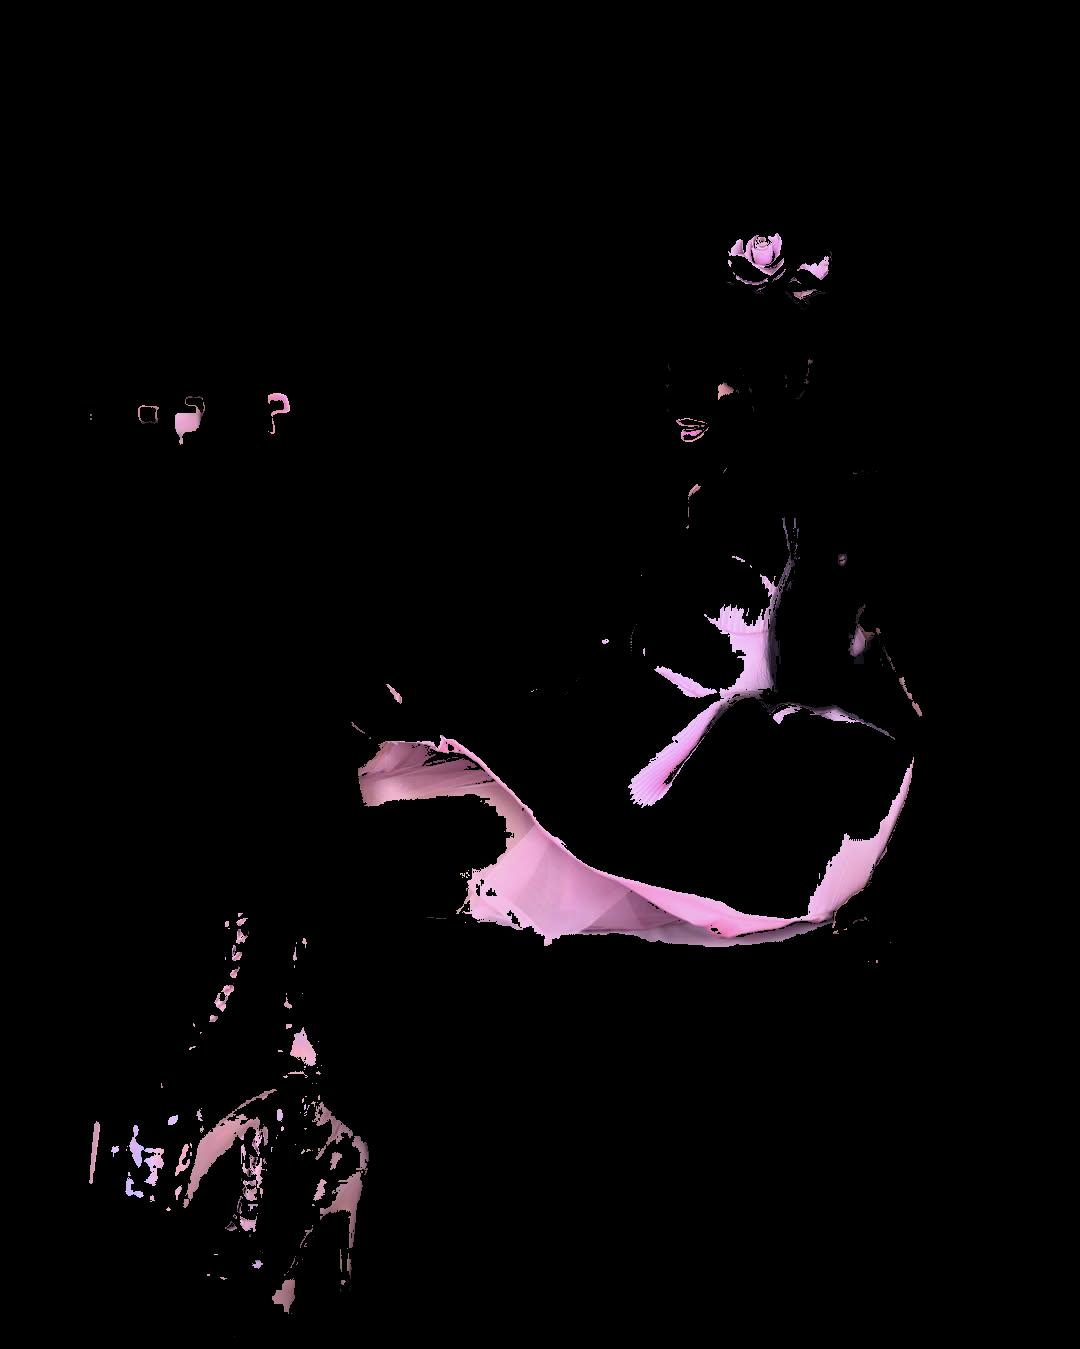
\includegraphics[width=\textwidth]{IMG/R13.jpg}
		\caption*{Mascara aplicada sobre la imagen original.}
	\end{minipage}
	\caption{Resultados de segmentar en HSV con umbral de 0.15.}
	\label{fig:f2}
\end{figure}

Los resultados para la segmentación con HSV y un umbral de 0.15, muestra solo aquellos pixeles que están muy parecidos a ese rosa intenso, pero aquellos que son un rosa más pálido por la iluminación como el que se muestra por la zona del abdomen

\newpage

\subsection{Segmentación en HSV con un umbral de 0.25}

\begin{figure}[h!]
	\centering
	\begin{minipage}{0.4\textwidth}
		\centering
		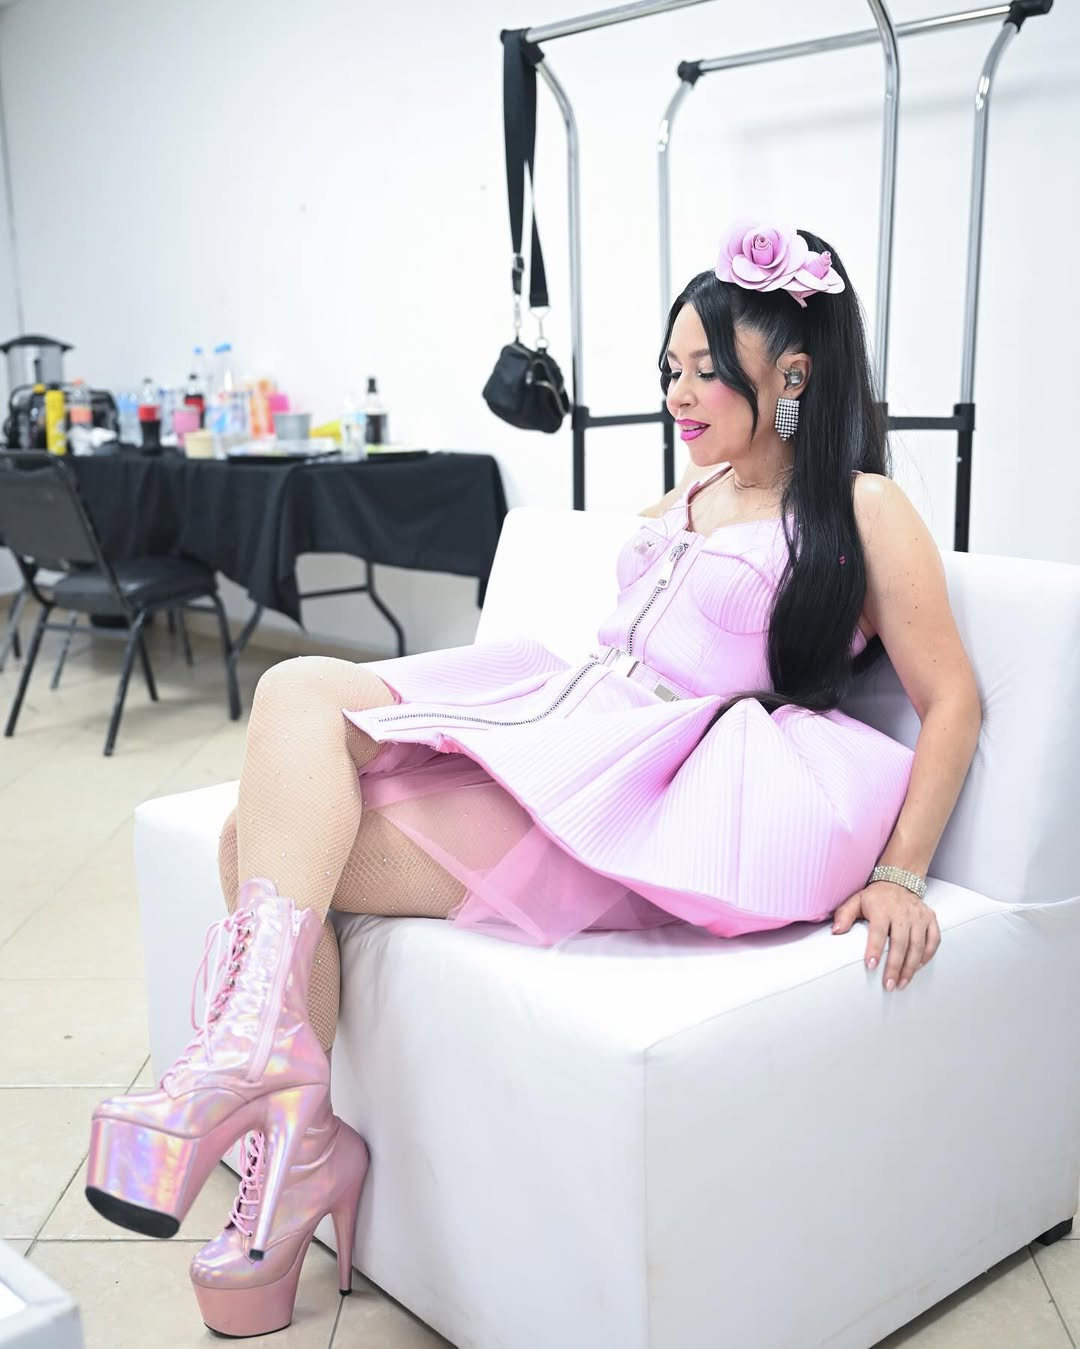
\includegraphics[width=\textwidth]{IMG/IM4.jpeg}
		\caption*{Imagen original.}
	\end{minipage}\hfill
	\begin{minipage}{0.4\textwidth}
		\centering
		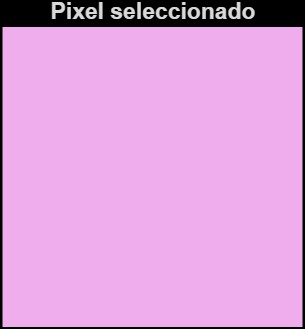
\includegraphics[width=\textwidth]{IMG/PIXEL.jpg}
		\caption*{Pixel seleccionado para la segmentación.}
	\end{minipage}
	
	\vspace{1em} % Espacio vertical entre las filas
	
	\begin{minipage}{0.4\textwidth}
		\centering
		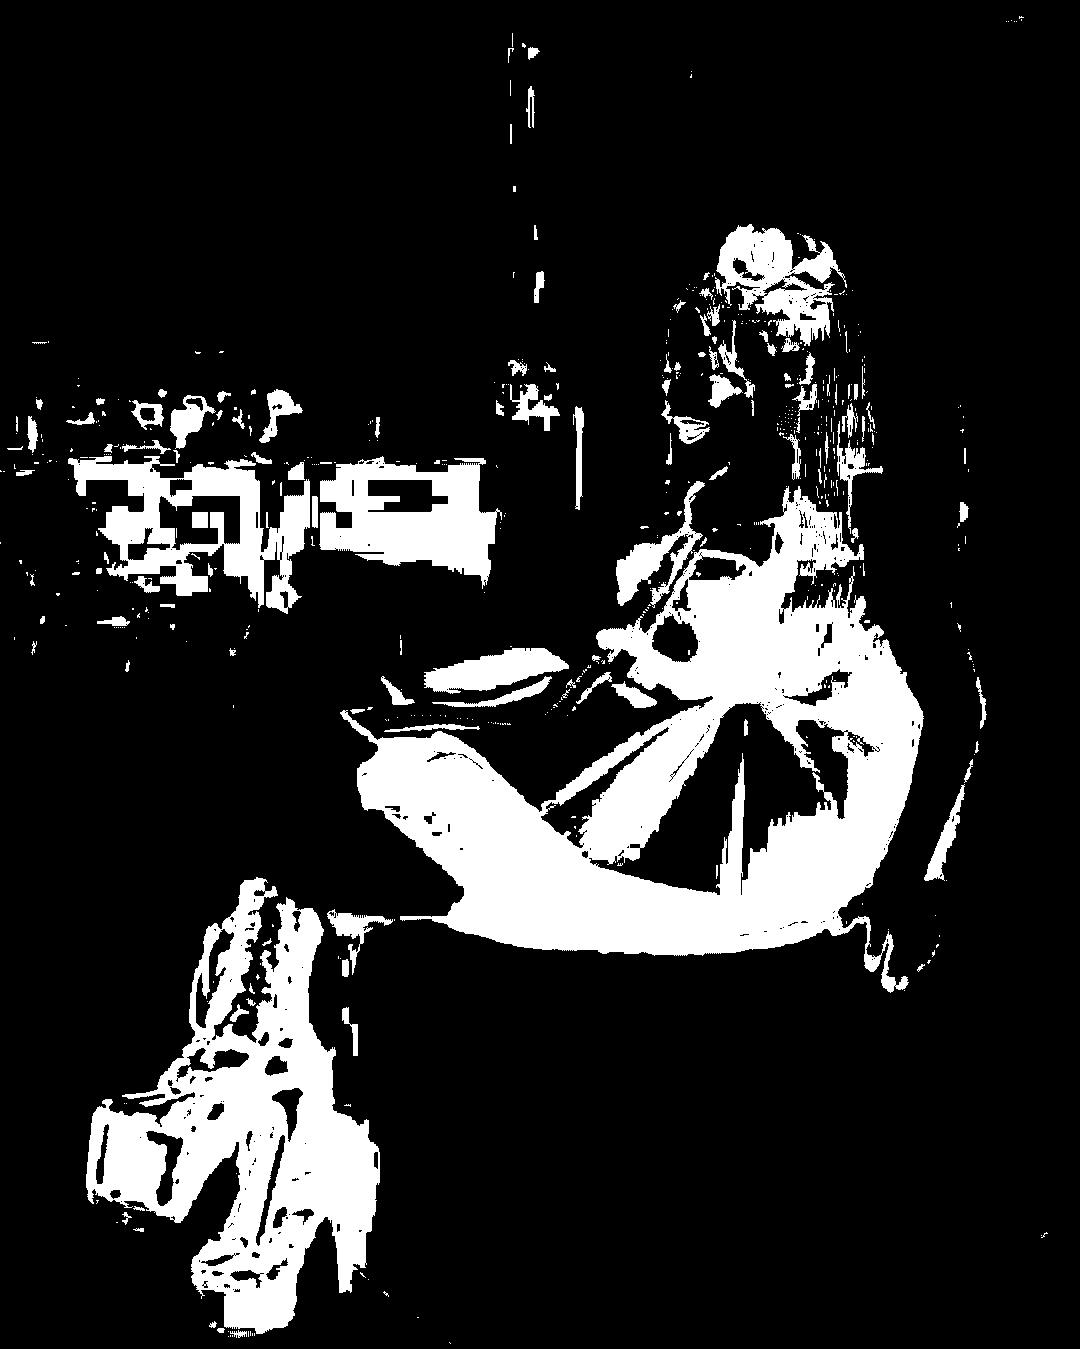
\includegraphics[width=\textwidth]{IMG/R22.jpg}
		\caption*{Mascara seleccionada.}
	\end{minipage}\hfill
	\begin{minipage}{0.4\textwidth}
		\centering
		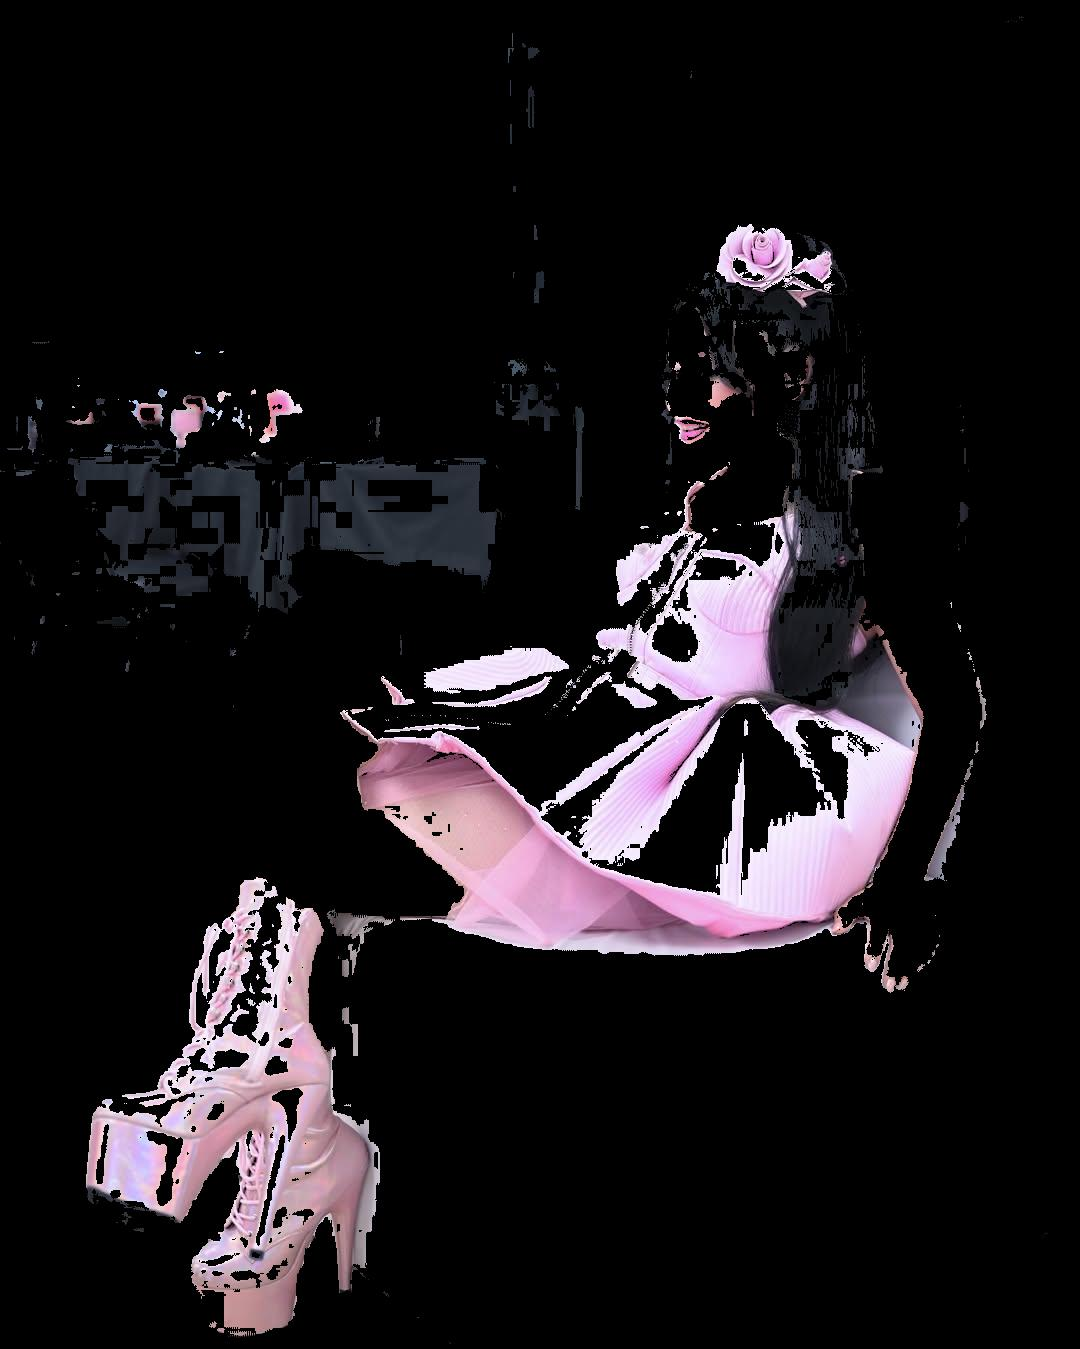
\includegraphics[width=\textwidth]{IMG/R23.jpg}
		\caption*{Mascara aplicada sobre la imagen original.}
	\end{minipage}
	\caption{Resultados de segmentar en HSV con umbral de 0.25.}
	\label{fig:f3}
\end{figure}

Los resultados de aumentar el umbral a 0.25 muestran con el mismo pixel de referencia, que detecta más tonalidades de rosa aunque sean más palidos por la luz, como lo es alrededor del vestido, los labios y las mejillas.

\newpage

\subsection{Segmentación en LAB con un umbral de 15}

\begin{figure}[h!]
	\centering
	\begin{minipage}{0.4\textwidth}
		\centering
		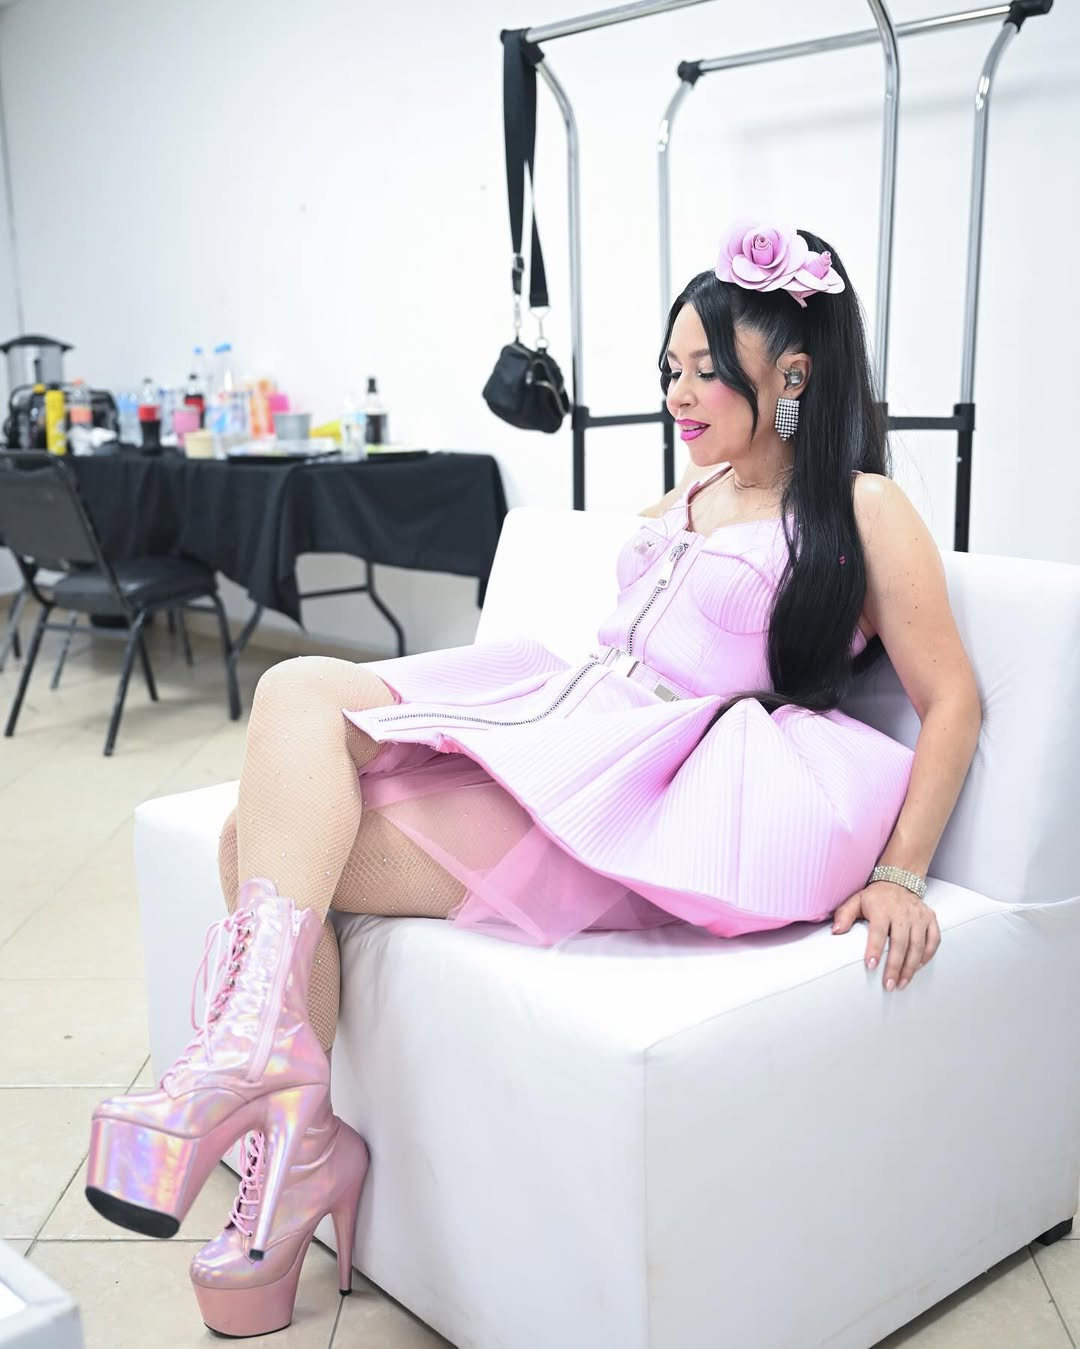
\includegraphics[width=\textwidth]{IMG/IM4.jpeg}
		\caption*{Imagen original.}
	\end{minipage}\hfill
	\begin{minipage}{0.4\textwidth}
		\centering
		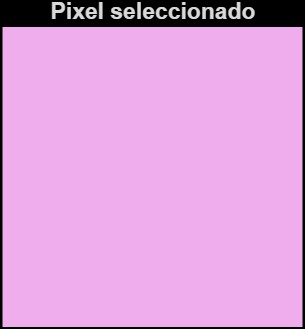
\includegraphics[width=\textwidth]{IMG/PIXEL.jpg}
		\caption*{Pixel seleccionado para la segmentación.}
	\end{minipage}
	
	\vspace{1em} % Espacio vertical entre las filas
	
	\begin{minipage}{0.4\textwidth}
		\centering
		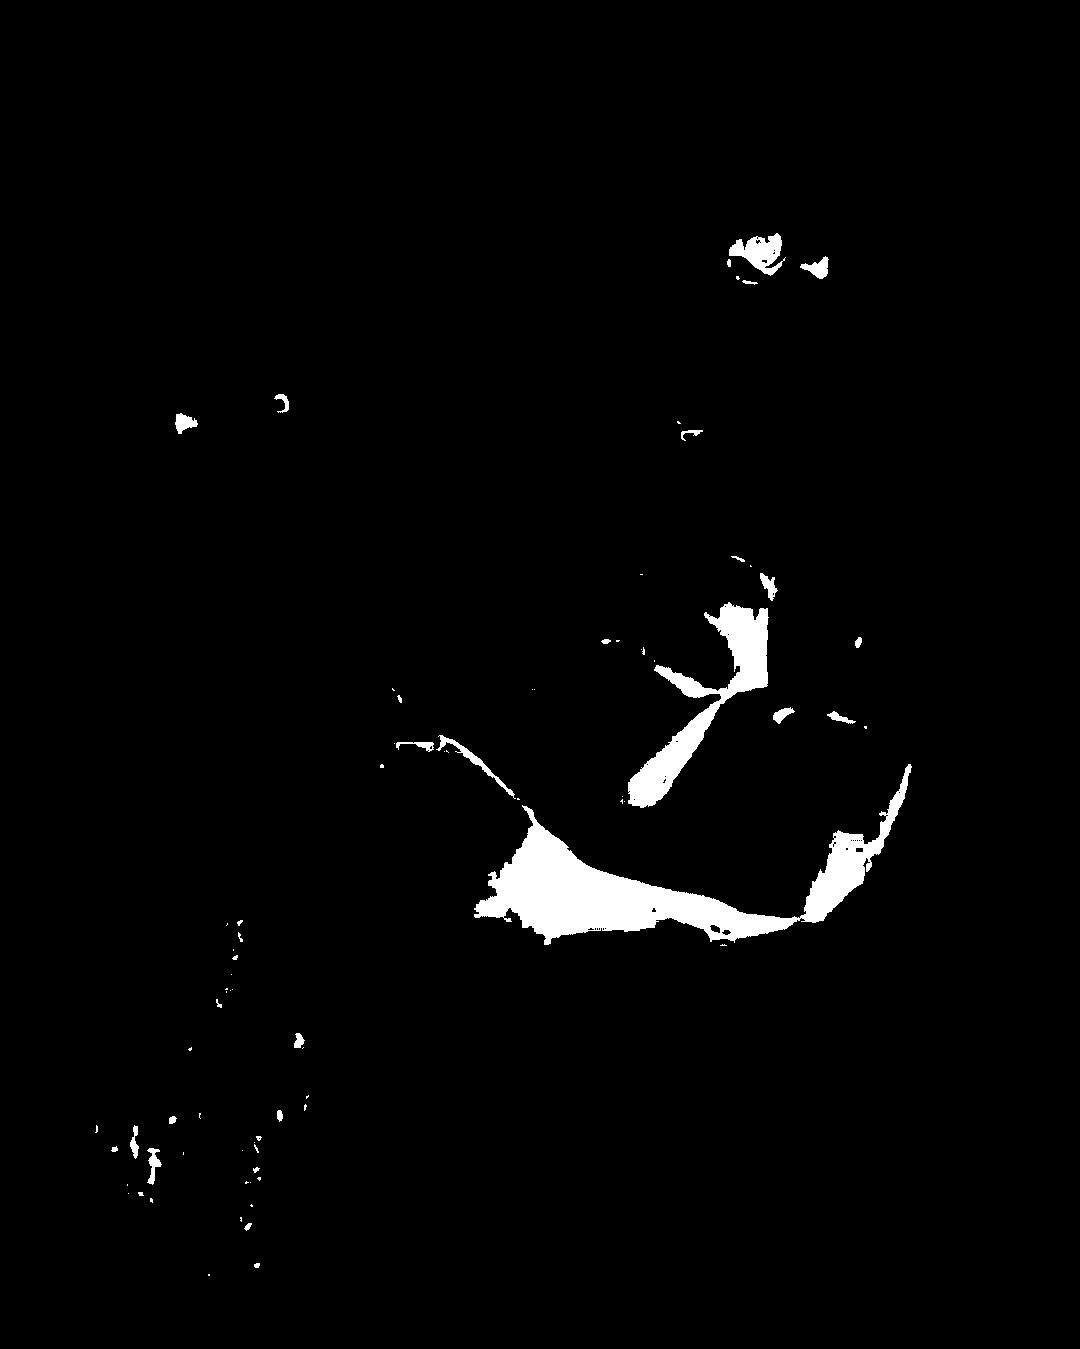
\includegraphics[width=\textwidth]{IMG/R32.jpg}
		\caption*{Mascara seleccionada.}
	\end{minipage}\hfill
	\begin{minipage}{0.4\textwidth}
		\centering
		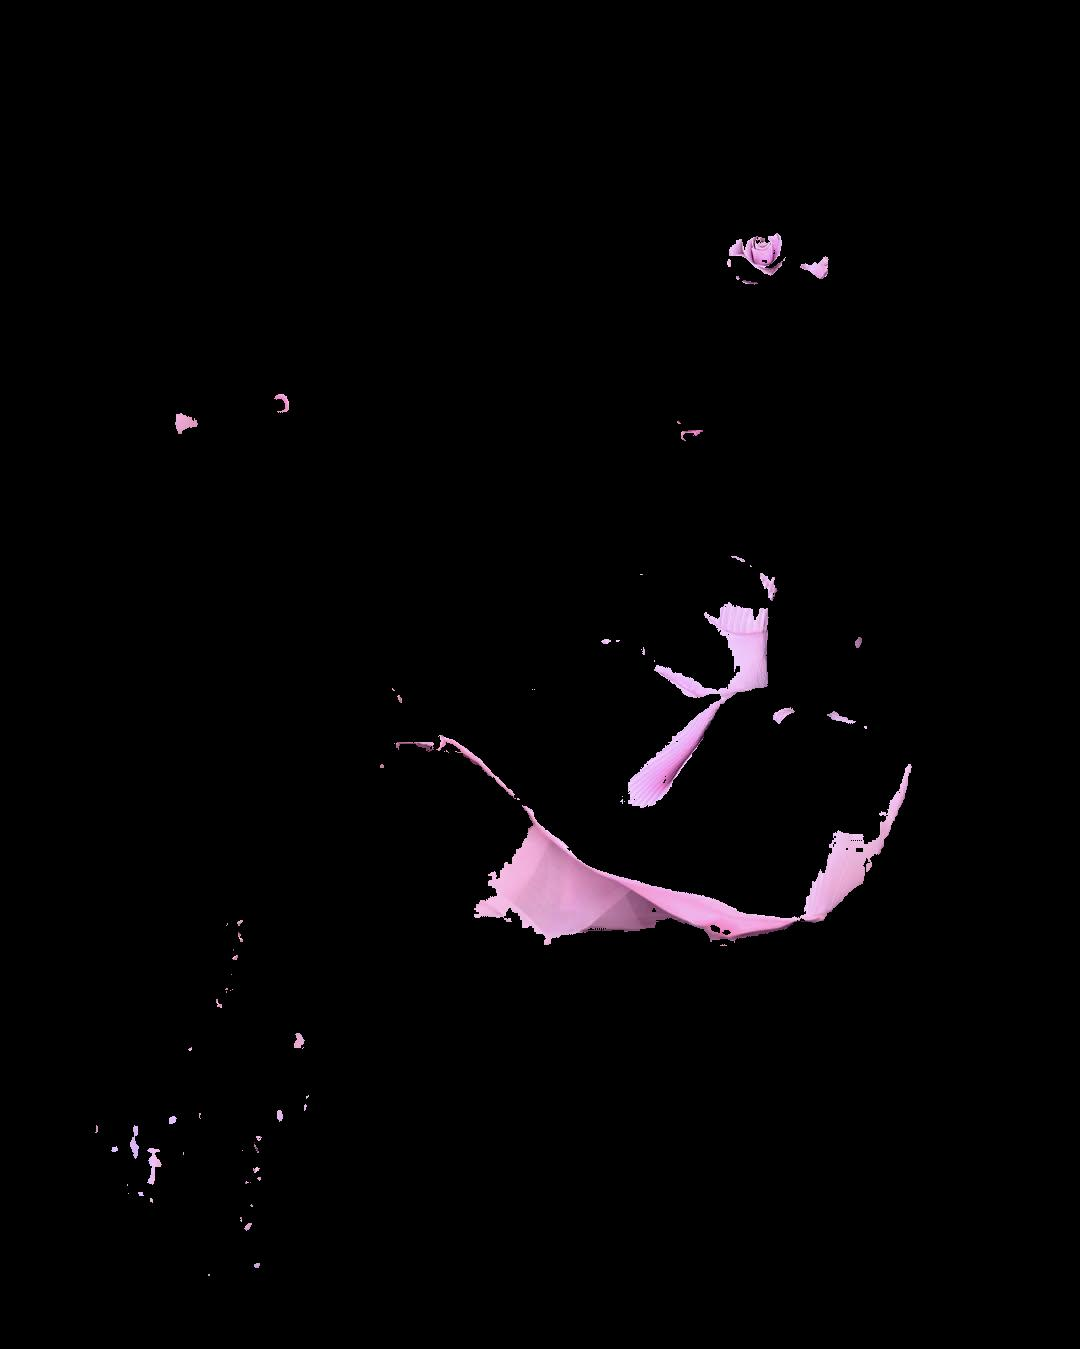
\includegraphics[width=\textwidth]{IMG/R33.jpg}
		\caption*{Mascara aplicada sobre la imagen original.}
	\end{minipage}
	\caption{Resultados de segmentar en LAB con umbral de 15.}
	\label{fig:f4}
\end{figure}

Al cambiar a el espacio LAB, con un umbral de 15 unidades, los resultados son muy  similares a los obtenidos en HSV con umbral de 0.15, solo que aquí detecta zonas más concretas, donde el rosa es más intenso.

\newpage

\subsection{Segmentación en LAB con un umbral de 25}

\begin{figure}[h!]
	\begin{minipage}{0.4\textwidth}
		\centering
		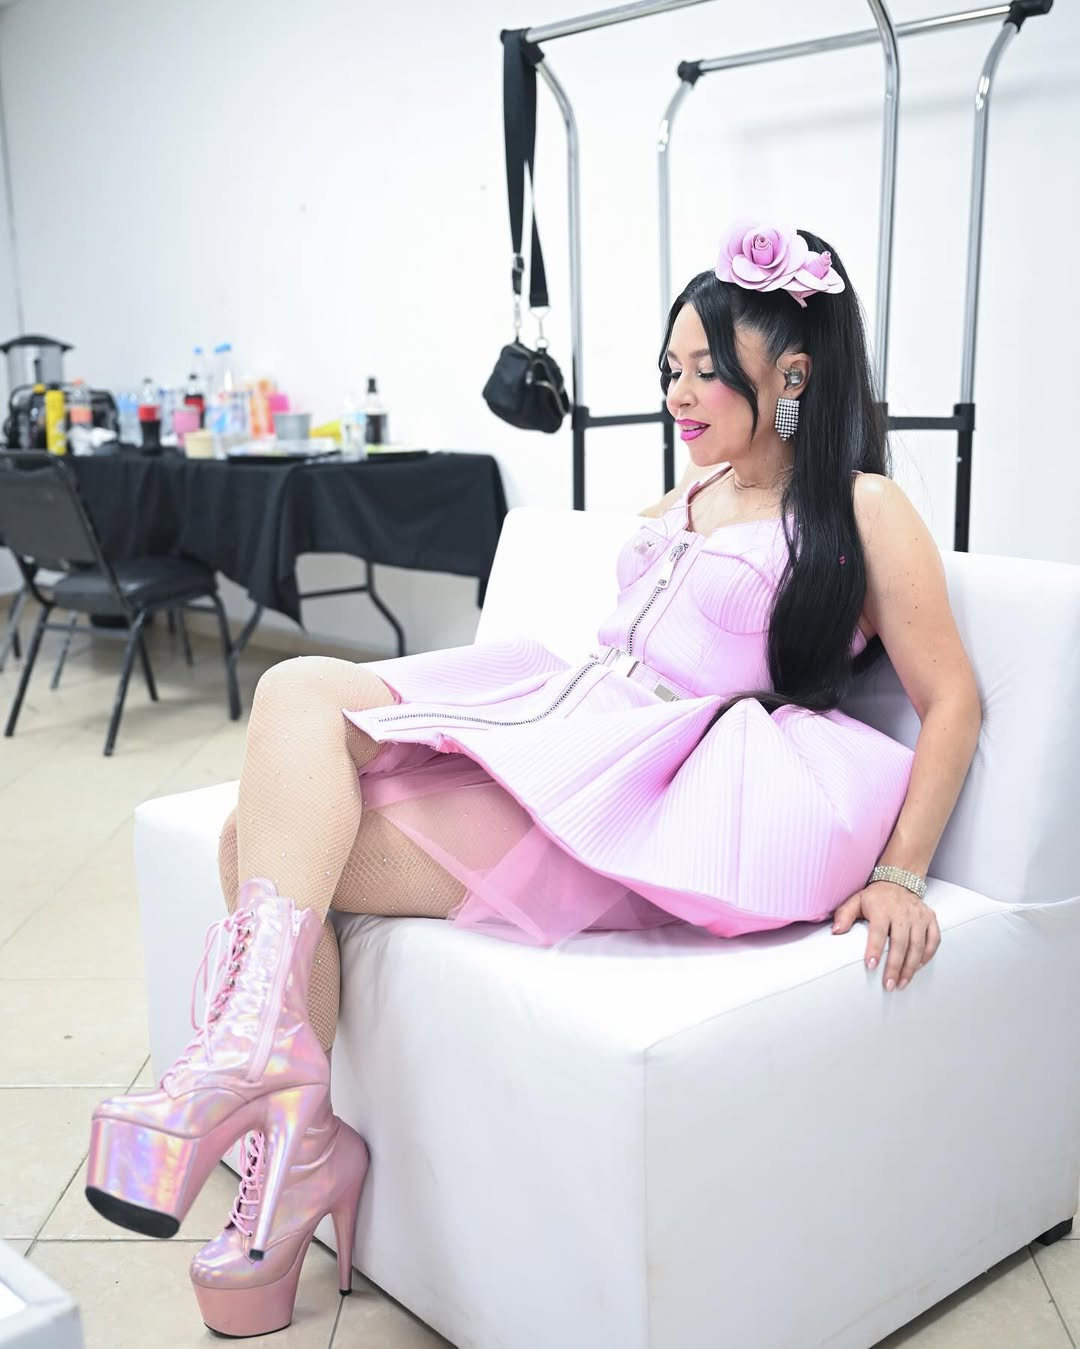
\includegraphics[width=\textwidth]{IMG/IM4.jpeg}
		\caption*{Imagen original.}
	\end{minipage}\hfill
	\begin{minipage}{0.4\textwidth}
		\centering
		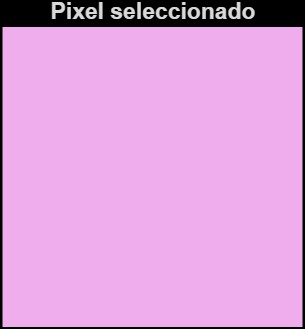
\includegraphics[width=\textwidth]{IMG/PIXEL.jpg}
		\caption*{Pixel seleccionado para la segmentación.}
	\end{minipage}
	
	\vspace{1em} % Espacio vertical entre las filas
	
	\begin{minipage}{0.4\textwidth}
		\centering
		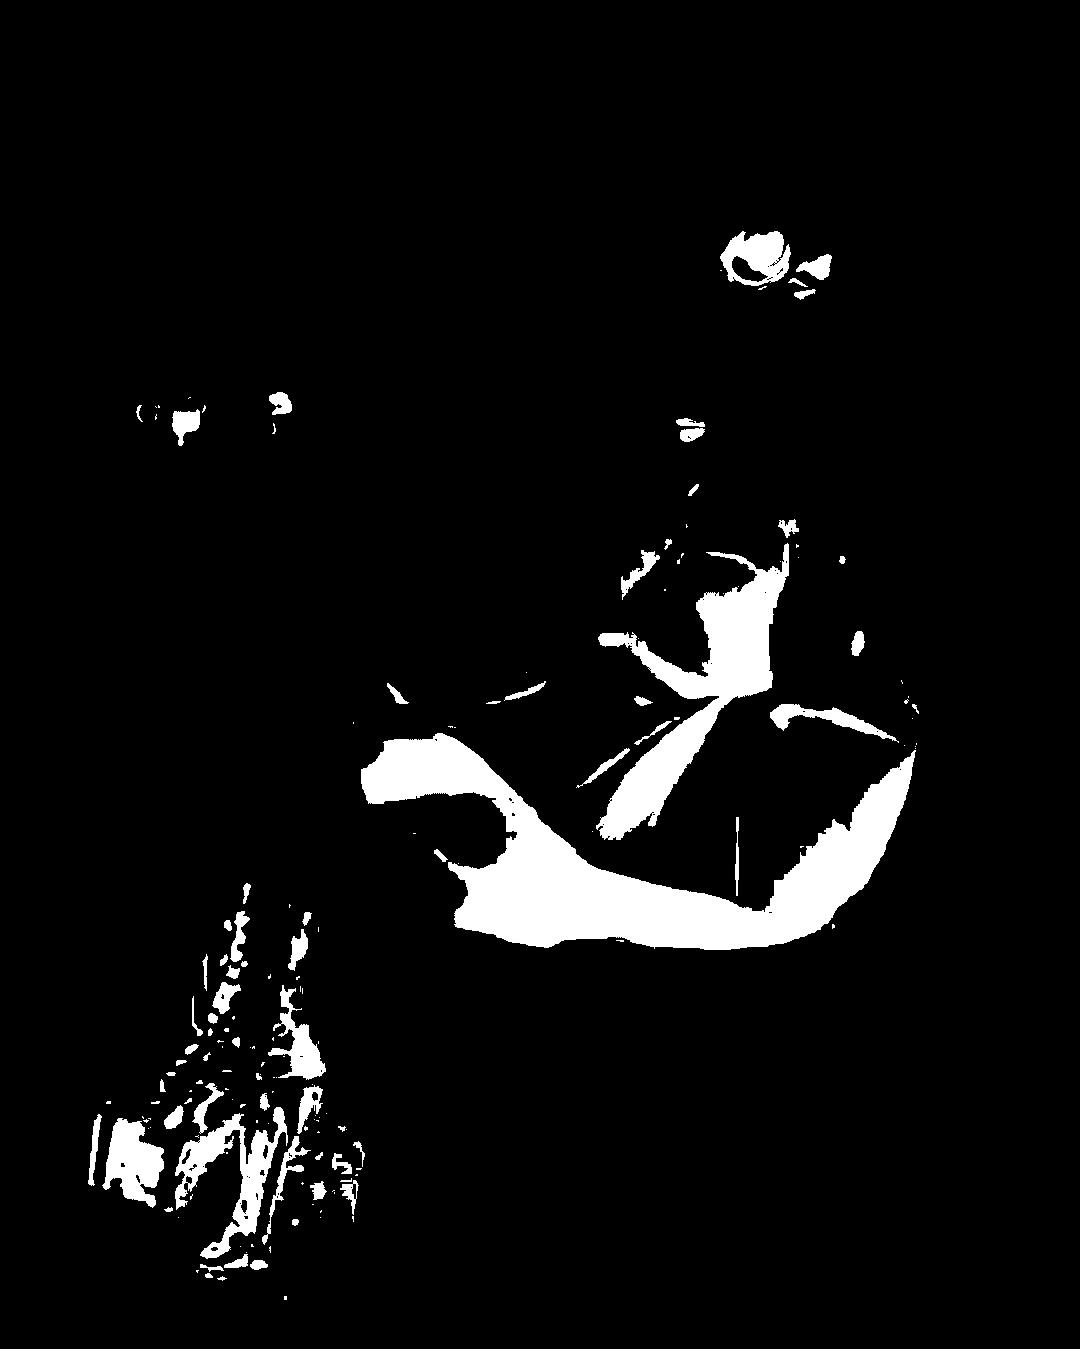
\includegraphics[width=\textwidth]{IMG/R42.jpg}
		\caption*{Mascara seleccionada.}
	\end{minipage}\hfill
	\begin{minipage}{0.4\textwidth}
		\centering
		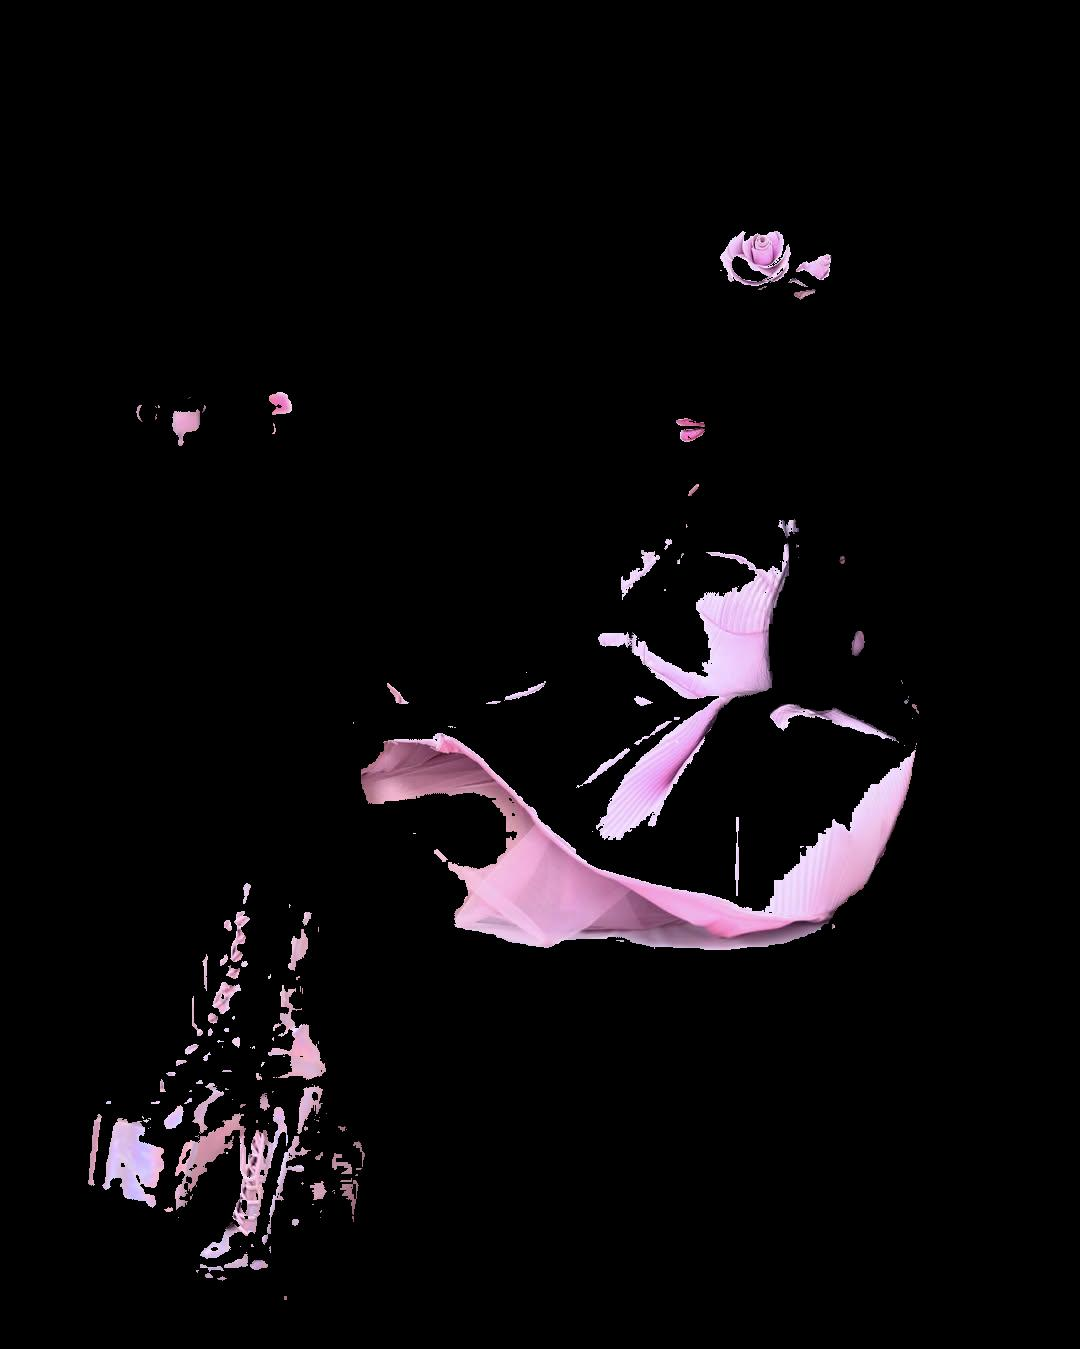
\includegraphics[width=\textwidth]{IMG/R43.jpg}
		\caption*{Mascara aplicada sobre la imagen original.}
	\end{minipage}
	\caption{Resultados de segmentar en LAB con umbral de 25.}
	\label{fig:f5}
\end{figure}

Al aumentar el umbral a 25 unidades, se nota encontrar como ahora encuentra más puntos en la imagen donde el rosa es más intenso, como en las botas, en los labios, el moño del cabello y elementos de la mesa.

\newpage

\subsection{Comparativa de la mascara resultante de los 4 experimentos}

\begin{figure}[h!]
	\begin{minipage}{0.4\textwidth}
		\centering
		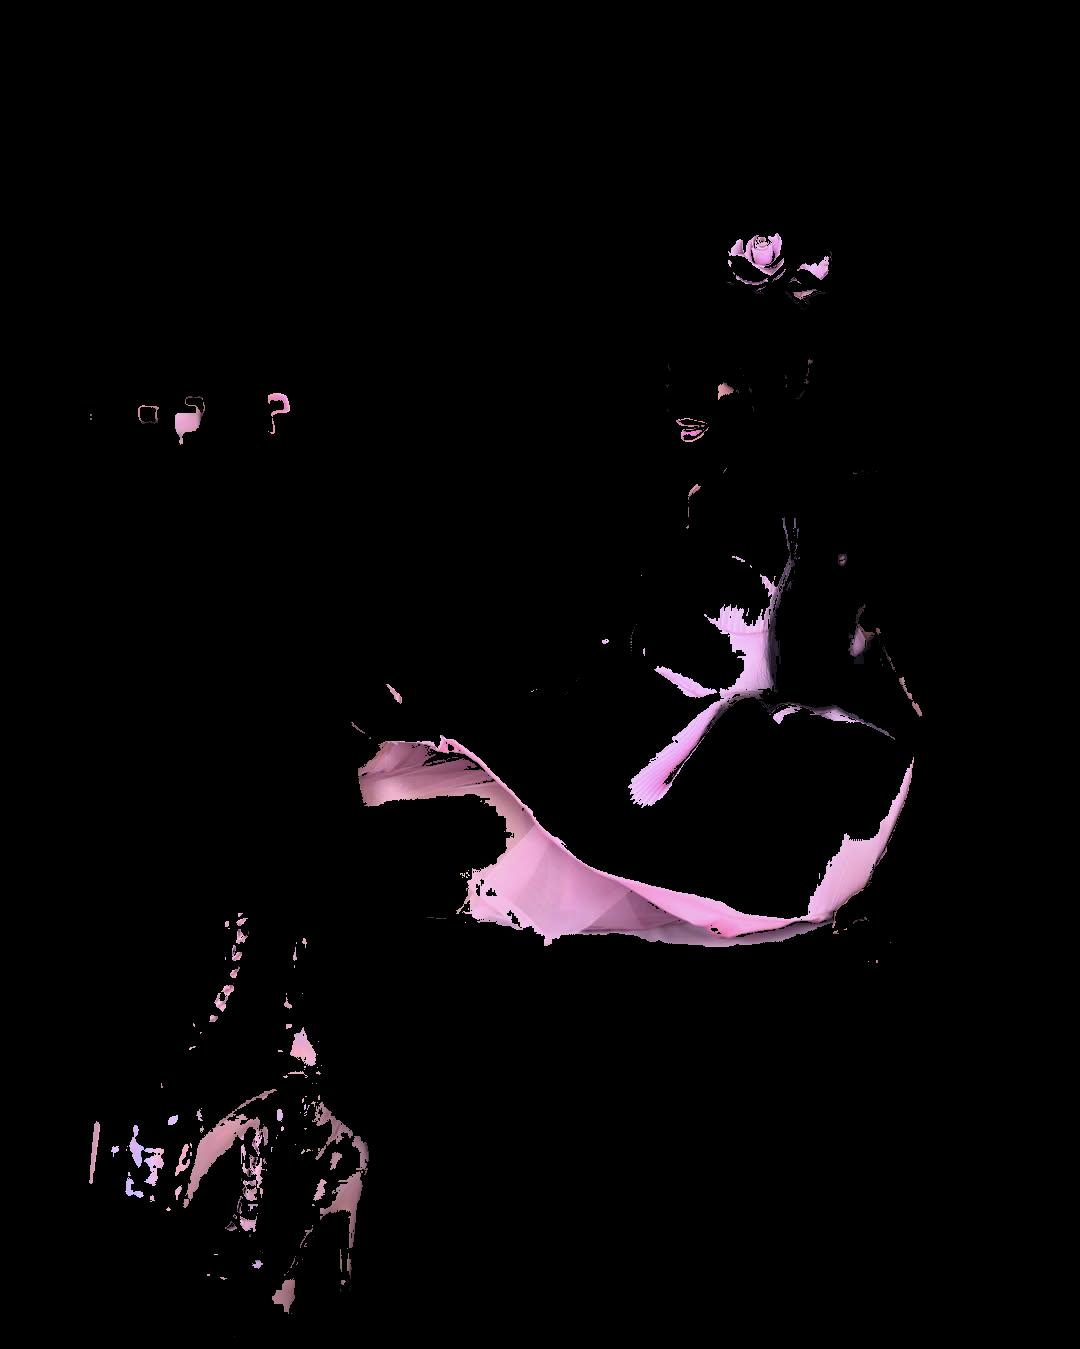
\includegraphics[width=\textwidth]{IMG/R13.jpg}
		\caption*{HSV con 0.15.}
	\end{minipage}\hfill
	\begin{minipage}{0.4\textwidth}
		\centering
		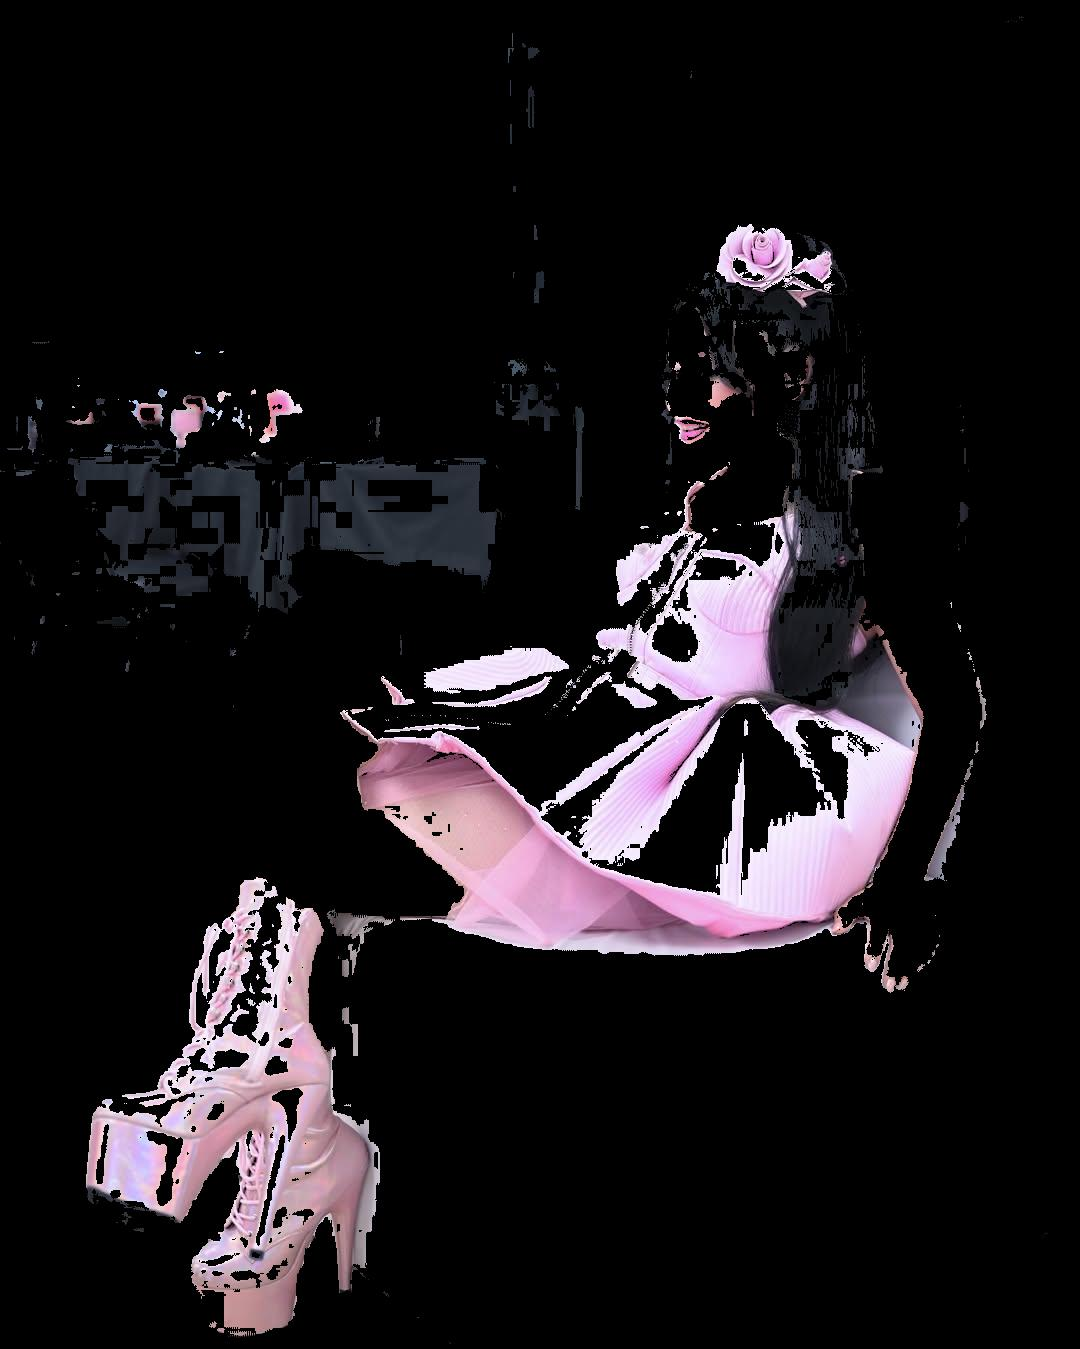
\includegraphics[width=\textwidth]{IMG/R23.jpg}
		\caption*{HSV con 0.25.}
	\end{minipage}
	
	\vspace{1em} % Espacio vertical entre las filas
	
	\begin{minipage}{0.4\textwidth}
		\centering
		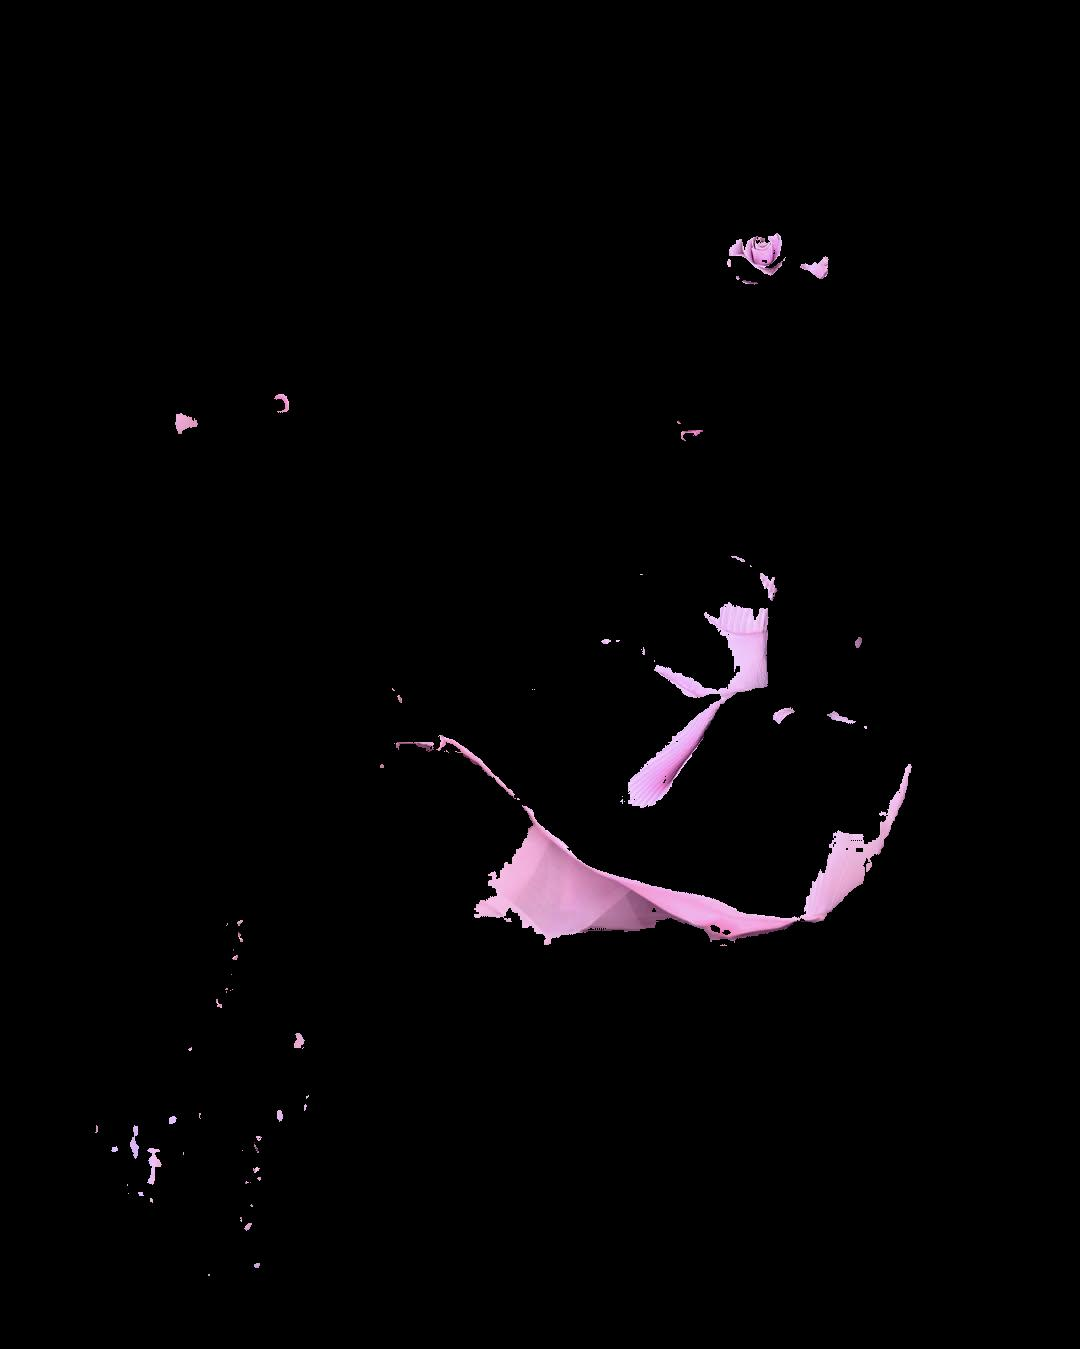
\includegraphics[width=\textwidth]{IMG/R33.jpg}
		\caption*{LAB con 15.}
	\end{minipage}\hfill
	\begin{minipage}{0.4\textwidth}
		\centering
		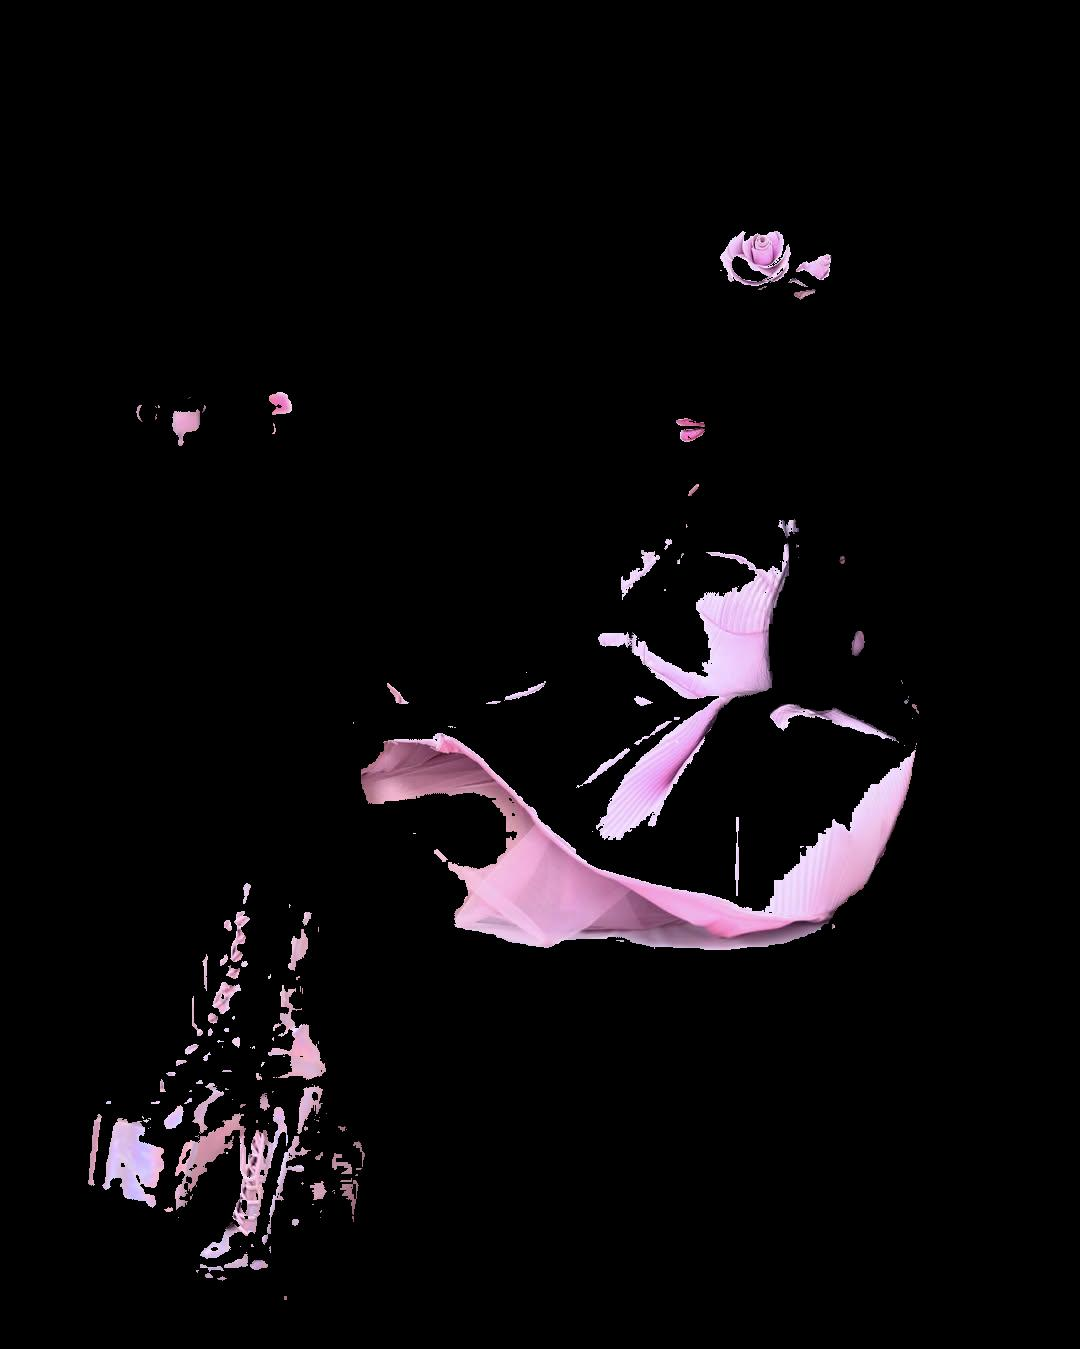
\includegraphics[width=\textwidth]{IMG/R43.jpg}
		\caption*{LAB con 25.}
	\end{minipage}
	\caption{Comparativa de las mascaras resultantes.}
	\label{fig:f6}
\end{figure}

Al mostrar la comparativa de las 4 mascaras obtenidas, salta a la vista que HSV con 0.25 de umbral encuentra más pixeles parecidos al rosa que LAB con 25.


\newpage
	
\section{Conclusiones}

Tras la implementación del algoritmo de segmentación y hacer el recorrido entre los espacios de color HSV y LAB, se llega a la conclusión de que son alternativas bastante potentes, al lograr esta separación de los canales de colores del brillo de la imagen, hecho que se ve reflejado en las mascaras obtenidas. Mientras que HSV logra detectar un mayor rango de pixeles dentro de la tonalidad de referencia, LAB encuentra conjuntos de pixeles más concretos respecto a su referencia.

\newpage

	
\section{Referencias}  % Sección numerada de referencias
\bibliographystyle{apalike}  % Estilo de citas (puedes cambiarlo)
\bibliography{Biblio}        % Nombre del archivo BibTeX (sin extensión)

\newpage
	
\section{Anexos}	
\subsection{Implementación de la segmentación para imagenes en HSV y LAB en MATLAB}
\begin{minted}[linenos,firstnumber=1]{matlab}
%% Distancia Euclideana %%
function d = distanciaE(x, y)
d = sqrt(sum((x - y).^2));
end

%% Función que transforma entre espacios
function [pixel, mascara, imgres] = SegEspacios(img, espacio, umbral)
%% Mostrar imagen y seleccionar pixel %%
fig = figure;
imshow(img);
title('Haz zoom (botón de lupa) y presiona ENTER cuando estés listo');
zoom on;
pause;
zoom off;
title('Ahora selecciona un pixel con un clic');
[col, fila] = ginput(1);
pixel = img(round(fila), round(col), :);
close(fig);
disp(['Coordenadas del pixel: x=', num2str(round(col)), ', y=', num2str(round(fila))]);
disp(['Color RGB: ', num2str(squeeze(pixel)')]);

%% Conversión al espacio de color hsv o lab %%
switch lower(espacio)
% CASO PARA HSV
case 'hsv'
img_convertido = rgb2hsv(img);
pixel_ref = rgb2hsv(pixel);
ref_vec = [pixel_ref(:,:,1), pixel_ref(:,:,2)];
A = img_convertido(:,:,1);
B = img_convertido(:,:,2);
% CASO PARA LAB
case 'lab'
img_convertido = rgb2lab(img);
pixel_ref = rgb2lab(pixel);
ref_vec = [pixel_ref(:,:,2), pixel_ref(:,:,3)];
A = img_convertido(:,:,2);
B = img_convertido(:,:,3);
otherwise
error('Espacio de color no válido. Usa "hsv" o "lab".');
end

%% Crear máscara basada en distancia euclideana %%
[n, p, ~] = size(img); % Obtener las dimensiones
mascara = zeros(n, p); % Crear la mascara vacia
% Identificar pixel a pixel si cumple o no el umbral
for i = 1:n
for j = 1:p
color_vec = [A(i,j), B(i,j)];
if distanciaE(color_vec, ref_vec) <= umbral
mascara(i,j) = 1;
end
end
end

%% Aplicar la máscara a la imagen %%
imgres = img;
imgres(repmat(~mascara, [1 1 3])) = 0;

%% Mostrar resultados %%
figure;
subplot(2,2,1); imshow(img); title('Imagen original');
subplot(2,2,2); imshow(pixel); title('Pixel seleccionado');
subplot(2,2,3); imshow(mascara); title('Máscara generada');
subplot(2,2,4); imshow(imgres); title('Imagen segmentada');
end


%% Cargar la imagen %%
ruta = "REPORTE\\IMG\\IM4.jpeg";
img = imread(ruta);

%% Pruebas para HSV color rosa umbral 0.15 %%
[pixel, mascara, imgres] = SegEspacios(img, "hsv", 0.15);
imwrite(pixel, "R11.jpg")
imwrite(mascara, "R12.jpg")
imwrite(imgres, "R13.jpg")
%% Pruebas para HSV color rosa umbral 0.25 %%
[pixel, mascara, imgres] = SegEspacios(img, "hsv", 0.25);
imwrite(pixel, "R21.jpg")
imwrite(mascara, "R22.jpg")
imwrite(imgres, "R23.jpg")
%% Pruebas para LAB color rosa umbral 15 %%
[pixel, mascara, imgres] = SegEspacios(img, "lab", 15);
imwrite(pixel, "R31.jpg")
imwrite(mascara, "R32.jpg")
imwrite(imgres, "R33.jpg")
%% Pruebas para LAB color rosa umbral 25 %%
[pixel, mascara, imgres] = SegEspacios(img, "lab", 25);
imwrite(pixel, "R41.jpg")
imwrite(mascara, "R42.jpg")
imwrite(imgres, "R43.jpg")
\end{minted}
	
	
	
	
\end{document}

